\chapter{Plateforme et Architecture Logicielle}

Le pipeline décrit au chapitre précédent est un enchaînement de traitements exécutés par un programme Python. Pour qu'il soit utilisable par les analystes de l'Office des Changes, il devait être intégré dans une plateforme web accessible, configurable et observable. Ce chapitre présente l'architecture logicielle de cette plateforme, la communication entre ses composants, le déroulement d'une exécution complète, et les fonctionnalités offertes à l'utilisateur final.

\section{Architecture globale}

La plateforme suit une architecture en couches séparées, avec trois composants applicatifs et deux bases de données. L'interface est une application monopage qui fournit à l'utilisateur les écrans de configuration, de lancement, de suivi et de visualisation. Le serveur d'API centralise la logique métier, l'authentification et la persistance des configurations, des exécutions et des résultats. Le worker d'exécution héberge le pipeline d'Entity Resolution et réalise les calculs lourds. Les données de référence et les déclarations sont lues dans la base source, tandis que les configurations, les exécutions et les entités résolues sont persistées dans la base de la plateforme. La figure suivante présente cette architecture avec les technologies et les ports de chaque composant.

\begin{figure}[H]
\centering
\begin{tikzpicture}[
  node distance=1.2cm,
  service/.style={rectangle, rounded corners=4pt, draw=black, thick, minimum width=3.4cm, minimum height=1.6cm, align=center, font=\footnotesize},
  frontend/.style={service, fill=blue!10, draw=blue!60!black},
  backend/.style={service, fill=violet!10, draw=violet!60!black},
  worker/.style={service, fill=orange!12, draw=orange!60!black},
  database/.style={service, fill=teal!10, draw=teal!60!black},
  external/.style={service, fill=red!8, draw=red!60!black, dashed},
  arr/.style={-{Latex[length=2mm]}, thick},
  port/.style={font=\scriptsize, text=gray!70!black}
]
\node[frontend] (fe) {Interface\\[-2pt]\scriptsize React et Vite\\[-2pt]\port{:5173}};
\node[backend, right=of fe] (be) {Serveur d'API\\[-2pt]\scriptsize Express.js\\[-2pt]\port{:3001}};
\node[worker, right=of be] (wo) {Worker\\[-2pt]\scriptsize FastAPI et Splink\\[-2pt]\port{:8001}};
\node[database, below=of be] (pg) {Base plateforme\\[-2pt]\scriptsize PostgreSQL\\[-2pt]\port{:5544}};
\node[external, below=of wo] (mssql) {Base source\\[-2pt]\scriptsize SQL Server\\[-2pt]\port{:1433}};
\draw[arr] (fe) -- node[above, font=\scriptsize] {REST} (be);
\draw[arr] (be) -- node[above, font=\scriptsize] {HTTP et JSON} (wo);
\draw[arr] (be) -- node[right, font=\scriptsize] {ORM} (pg);
\draw[arr, dashed] (wo) -- node[right, font=\scriptsize] {ODBC} (mssql);
\draw[arr, dashed] (wo) -- node[above, font=\scriptsize] {Résultats} (pg);
\end{tikzpicture}
\caption{Architecture globale de la plateforme : une interface web, un serveur d'API, un worker de calcul, la base de la plateforme et la base source des déclarations.}
\label{fig:arch-globale}
\end{figure}

Cette séparation en couches présente plusieurs avantages. Les responsabilités sont clairement réparties : l'interface gère l'expérience utilisateur, le serveur d'API gère la logique métier et la persistance, et le worker gère le calcul intensif. Le worker peut être déployé sur une machine distincte dotée de davantage de mémoire sans modifier le reste du système, ce qui est précieux pour les étapes gourmandes telles que l'entraînement EM ou le calcul des plongements. Chaque composant peut également évoluer indépendamment tant que les contrats d'interface entre eux sont respectés.

En contrepartie, cette architecture impose de maintenir la cohérence de l'état du système entre les composants : une exécution existe à la fois comme enregistrement en base, comme traitement actif dans le worker et comme affichage dans l'interface. Le diagnostic des incidents nécessite donc de suivre le flux d'une requête à travers les trois couches, ce que le suivi temps réel des exécutions facilite.

\section{Le serveur d'API}

Le serveur d'API est développé avec le framework Express sur la plateforme Node.js, avec un typage strict en TypeScript. Il expose des routes REST pour la gestion des sources de données avec création, lecture, modification et suppression, pour la configuration des pipelines avec les règles de comparaison, les règles de blocage et les paramètres d'entraînement, pour le lancement et le suivi des exécutions, pour la consultation paginée des entités et des paires de correspondances, et pour la recherche intelligente d'opérateurs.

La persistance est assurée par une base PostgreSQL accédée via un ORM typé, ce qui garantit la cohérence entre le schéma de la base et le code de l'application. Les mots de passe des sources de données sont chiffrés par un algorithme symétrique robuste avant leur stockage, avec une clé fournie par variable d'environnement, de sorte qu'une lecture directe de la base ne révèle jamais d'identifiants en clair. L'authentification des utilisateurs repose sur des jetons signés qui accompagnent chaque requête.

\section{Le worker d'exécution}

Le worker est développé en Python avec le framework FastAPI. Il reçoit du serveur d'API la configuration complète d'une exécution, déroule les neuf étapes du pipeline décrites au chapitre précédent, et renvoie le résultat avec les métriques de chaque étape. Pendant l'exécution, il émet des événements de progression que le serveur d'API persiste et que l'interface interroge régulièrement, ce qui permet d'afficher une barre d'avancement et des journaux en temps réel.

Le worker gère également un cache des plongements neuronaux sur disque, afin d'éviter de recalculer les vecteurs lorsque les mêmes données et le même modèle sont réutilisés d'une exécution à l'autre. Les modèles de plongement sont téléchargés une seule fois et conservés localement. En cas d'erreur à une étape, l'exécution est marquée en échec avec le message d'erreur détaillé, et les étapes déjà accomplies restent consultables pour le diagnostic.

\section{Déroulement d'une exécution complète}

La figure suivante présente le diagramme de séquence d'une exécution de pipeline, depuis l'action de l'utilisateur jusqu'à la disponibilité des entités dans l'interface.

\begin{figure}[H]
\centering
\begin{tikzpicture}[
  participant/.style={rectangle, draw=black, thick, fill=gray!10, minimum width=2.4cm, minimum height=0.7cm, align=center, font=\footnotesize},
  lifeline/.style={dashed, gray},
  msg/.style={-{Latex[length=2mm]}, thick},
  lbl/.style={font=\scriptsize, align=center},
  note/.style={rectangle, draw=gray, fill=yellow!8, font=\scriptsize, align=left, inner sep=3pt}
]
\node[participant] (u) at (0, 0) {Utilisateur};
\node[participant] (f) at (3.1, 0) {Interface};
\node[participant] (a) at (6.2, 0) {Serveur d'API};
\node[participant] (w) at (9.3, 0) {Worker};
\node[participant] (b) at (12.4, 0) {Bases};
\draw[lifeline] (u) -- (0, -9.5);
\draw[lifeline] (f) -- (3.1, -9.5);
\draw[lifeline] (a) -- (6.2, -9.5);
\draw[lifeline] (w) -- (9.3, -9.5);
\draw[lifeline] (b) -- (12.4, -9.5);
\draw[msg] (0, -1.2) -- node[above, lbl] {Lancer le pipeline} (3.1, -1.2);
\draw[msg] (3.1, -2.0) -- node[above, lbl] {Créer l'exécution} (6.2, -2.0);
\draw[msg] (6.2, -2.8) -- node[above, lbl] {Transmettre la configuration} (9.3, -2.8);
\draw[msg] (9.3, -3.8) -- node[above, lbl] {Lire les déclarations} (12.4, -3.8);
\node[note] at (9.3, -4.9) {Nettoyage, normalisation, Splink,};
\node[note] at (9.3, -5.4) {embeddings, clustering, entités.};
\draw[msg] (9.3, -6.3) -- node[above, lbl] {Écrire entités et paires} (12.4, -6.3);
\draw[msg] (9.3, -7.1) -- node[above, lbl] {Résultat et métriques} (6.2, -7.1);
\draw[msg] (6.2, -7.9) -- node[above, lbl] {Suivi de progression} (3.1, -7.9);
\draw[msg] (3.1, -8.7) -- node[above, lbl] {Entités disponibles} (0, -8.7);
\end{tikzpicture}
\caption{Diagramme de séquence d'une exécution de pipeline : l'utilisateur lance le traitement depuis l'interface, le serveur d'API délègue au worker, le worker lit les déclarations, exécute les neuf étapes, persiste les résultats, et l'interface affiche les entités obtenues.}
\label{fig:sequence}
\end{figure}

Le suivi de l'exécution s'effectue par interrogation régulière de l'état de l'exécution : l'interface demande périodiquement au serveur d'API l'avancement courant, que le worker met à jour à chaque étape dans la base de la plateforme. L'annulation est gérée par un indicateur en base que le worker vérifie aux points de contrôle, ce qui permet d'interrompre proprement une exécution devenue inutile.

\section{Fonctionnalités de l'interface}

\subsection{Configuration des pipelines}

L'interface permet de déclarer les sources de données avec leurs paramètres de connexion, de sélectionner la table et les colonnes à traiter, de définir les règles de comparaison et de blocage de Splink avec leurs seuils, de régler les paramètres de l'entraînement EM, d'activer ou non l'étape d'embeddings avec le modèle et la pondération, et de choisir la stratégie de clustering avec ses paramètres. Chaque pipeline ainsi configuré peut être réutilisé pour des exécutions successives, ce qui favorise la reproductibilité des traitements.

\begin{figure}[H]
\centering
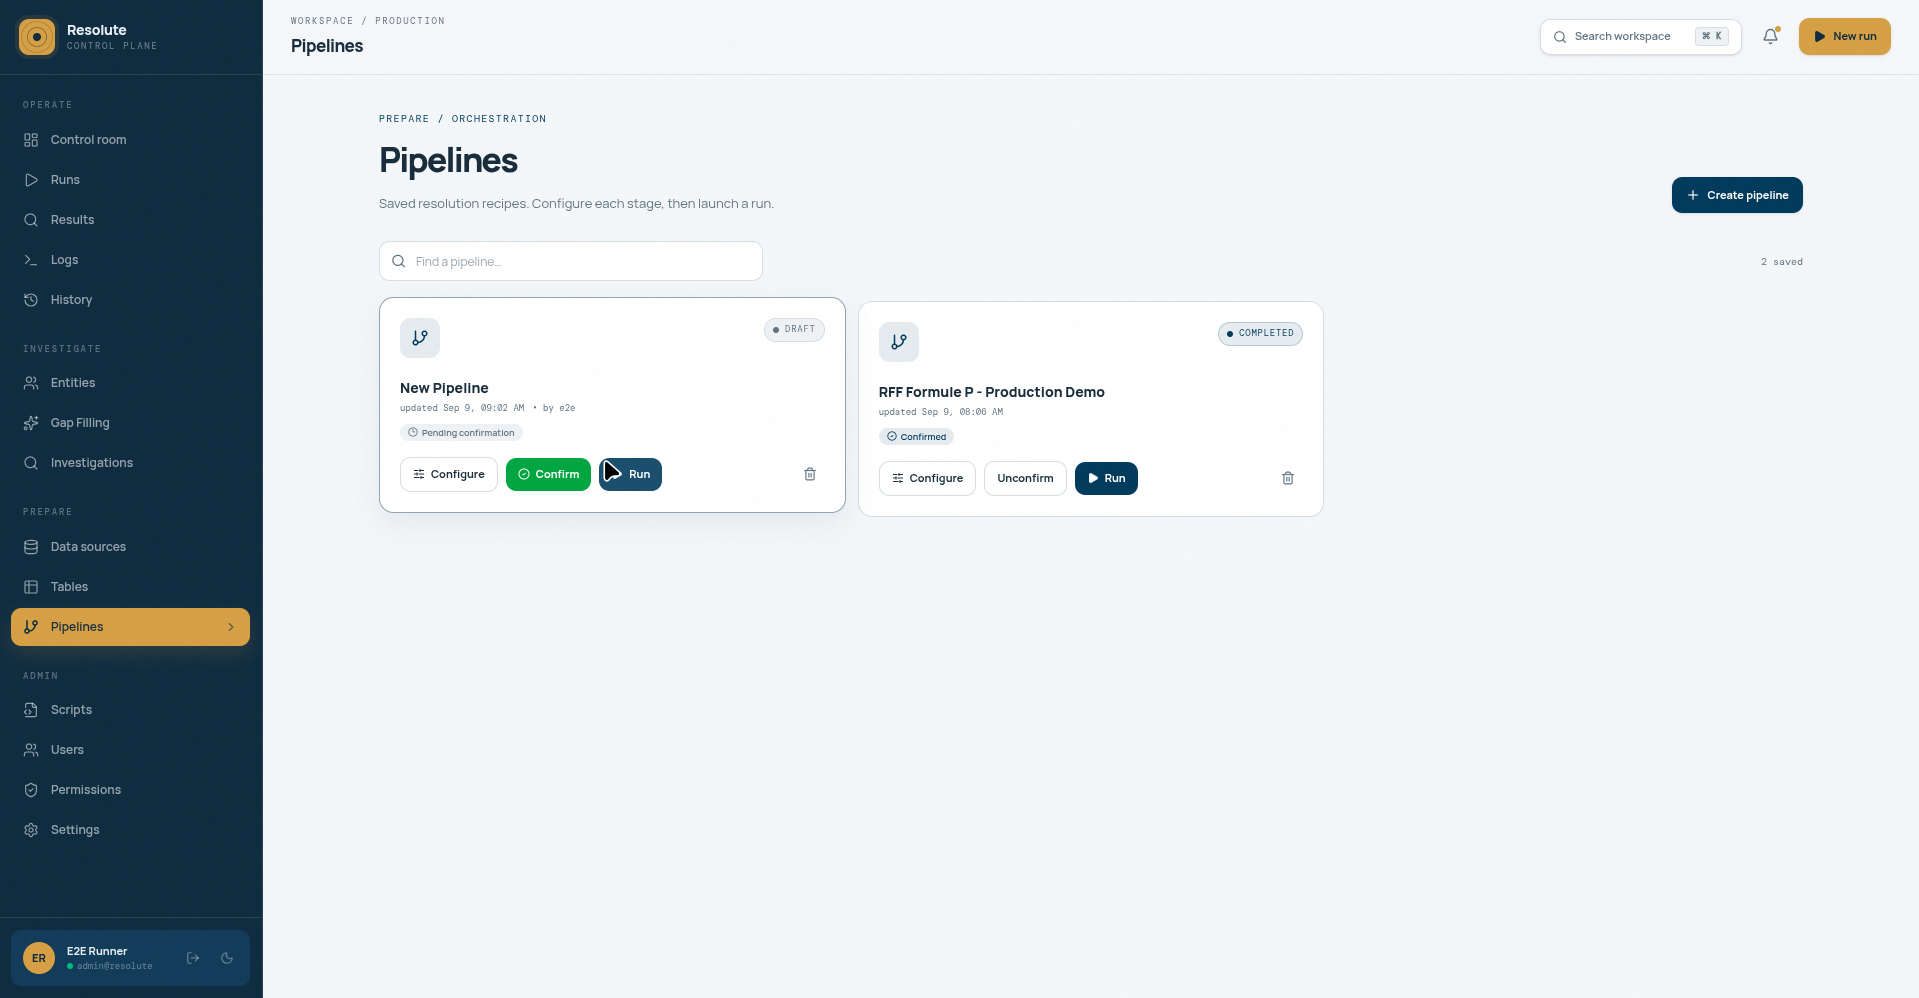
\includegraphics[width=0.9\textwidth]{images/screenshots/pipelines_page.png}
\caption{Page des pipelines : liste des pipelines configurés avec leur état et leurs actions disponibles.}
\label{fig:shot-pipelines}
\end{figure}

\begin{figure}[H]
\centering
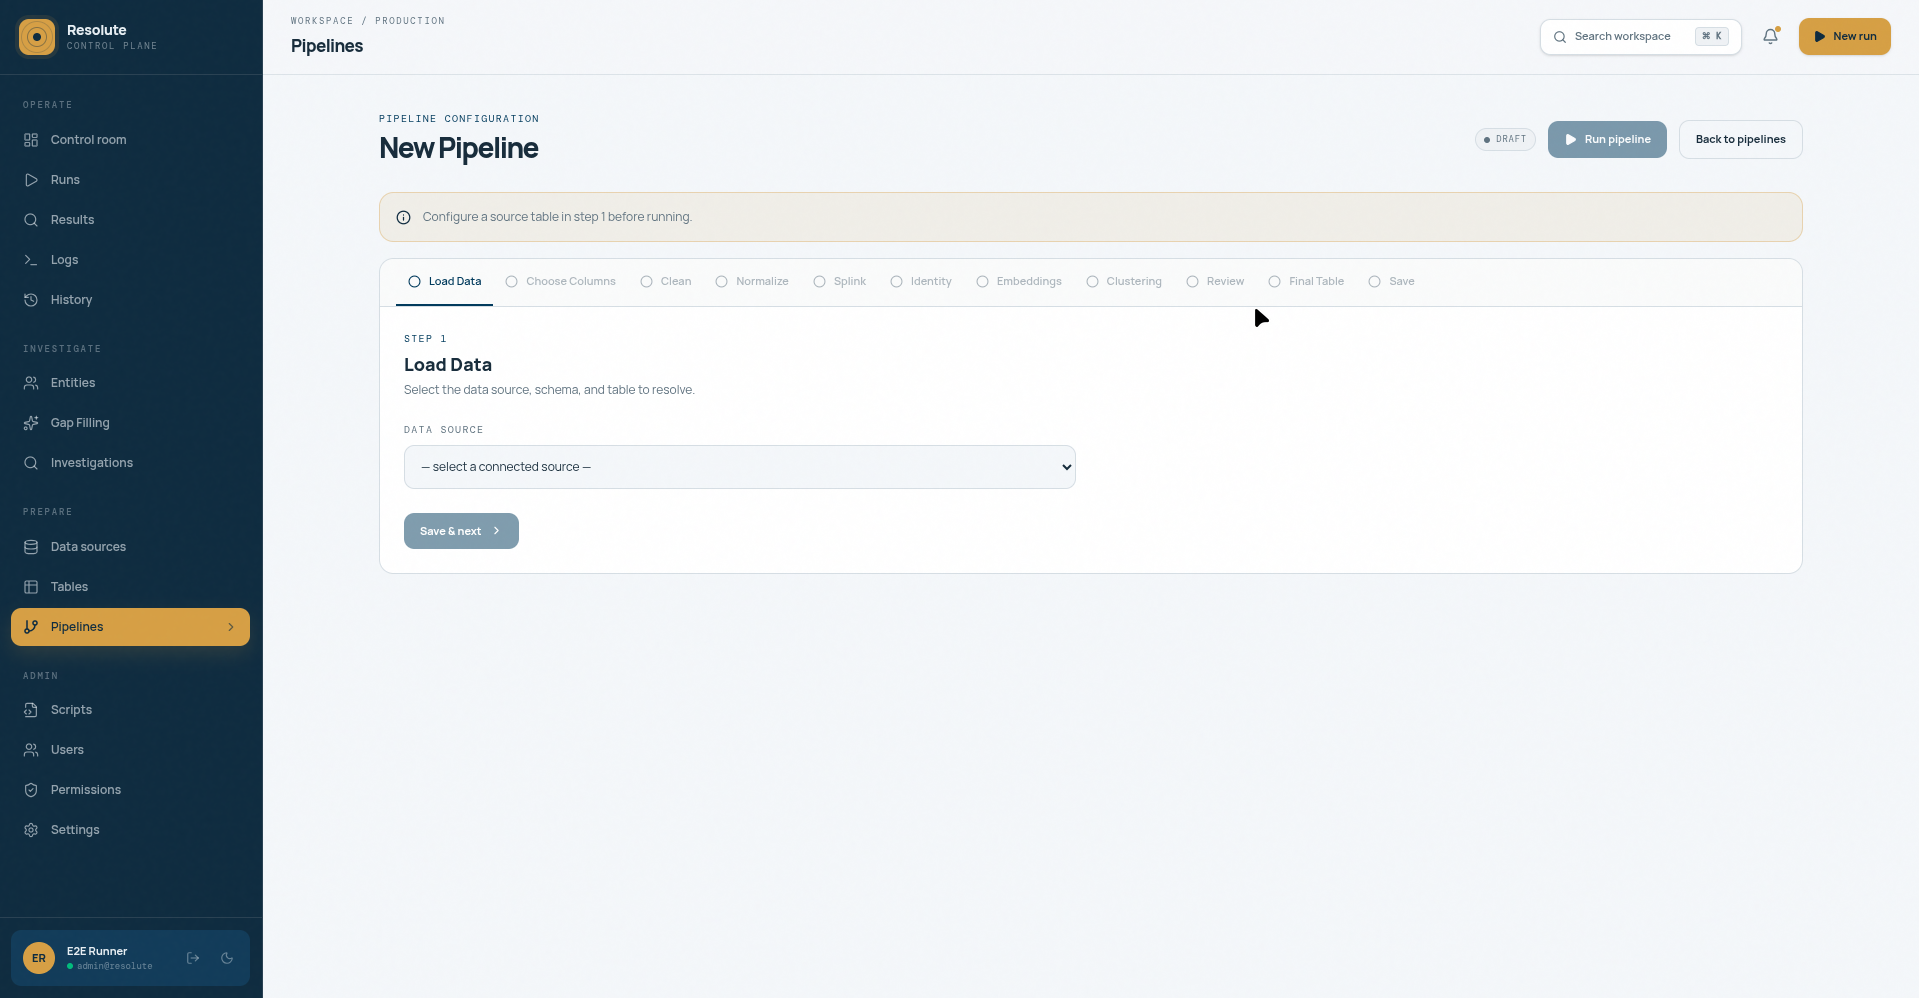
\includegraphics[width=0.9\textwidth]{images/screenshots/pipeline_creation.png}
\caption{Écran de création d'un pipeline : sélection de la source, de la table et des colonnes à traiter.}
\label{fig:shot-creation}
\end{figure}

\subsection{Suivi des exécutions}

Chaque exécution dispose d'une page de détail qui présente son statut global, la progression étape par étape avec les durées et les volumes traités, les métriques produites par Splink telles que le nombre de paires candidates et retenues, et les journaux d'événements émis par le worker. En cas d'échec, le message d'erreur et l'étape concernée sont mis en évidence pour faciliter le diagnostic.

\begin{figure}[H]
\centering
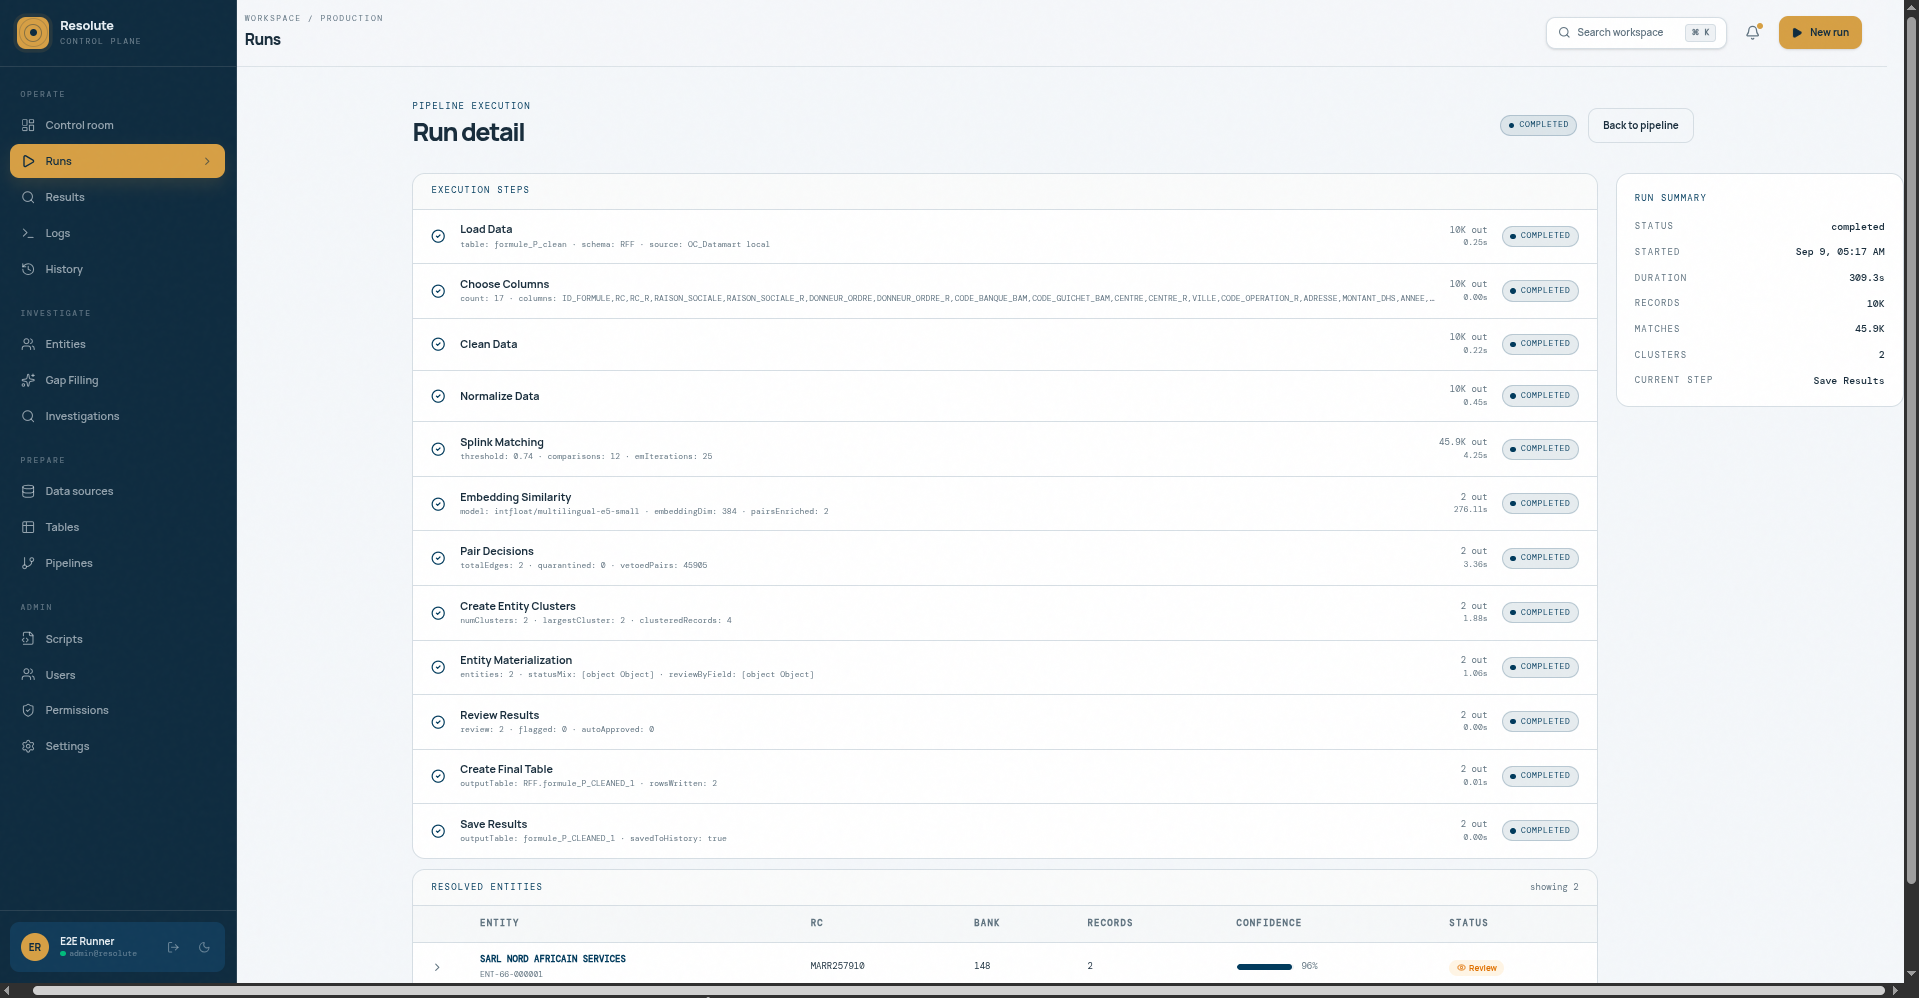
\includegraphics[width=0.9\textwidth]{images/screenshots/pipeline_execution.png}
\caption{Suivi d'une exécution de pipeline : avancement étape par étape avec les volumes traités.}
\label{fig:shot-execution}
\end{figure}

\subsection{Visualisation des entités}

La page des entités présente la liste des opérateurs identifiés par le pipeline. Chaque ligne affiche l'identifiant de l'entité, son nom canonique, ses codes de banque et de guichet, le nombre de déclarations qui lui sont rattachées et son statut. Le statut est matérialisé par un code couleur : les entités de confiance élevée sont approuvées automatiquement, les entités de confiance intermédiaire sont proposées à la révision, et les entités de faible confiance ou de taille anormale sont signalées. La fiche détaillée d'une entité présente l'ensemble de ses déclarations avec leurs champs, en distinguant les versions déclarées et corrigées des identifiants.

\begin{figure}[H]
\centering
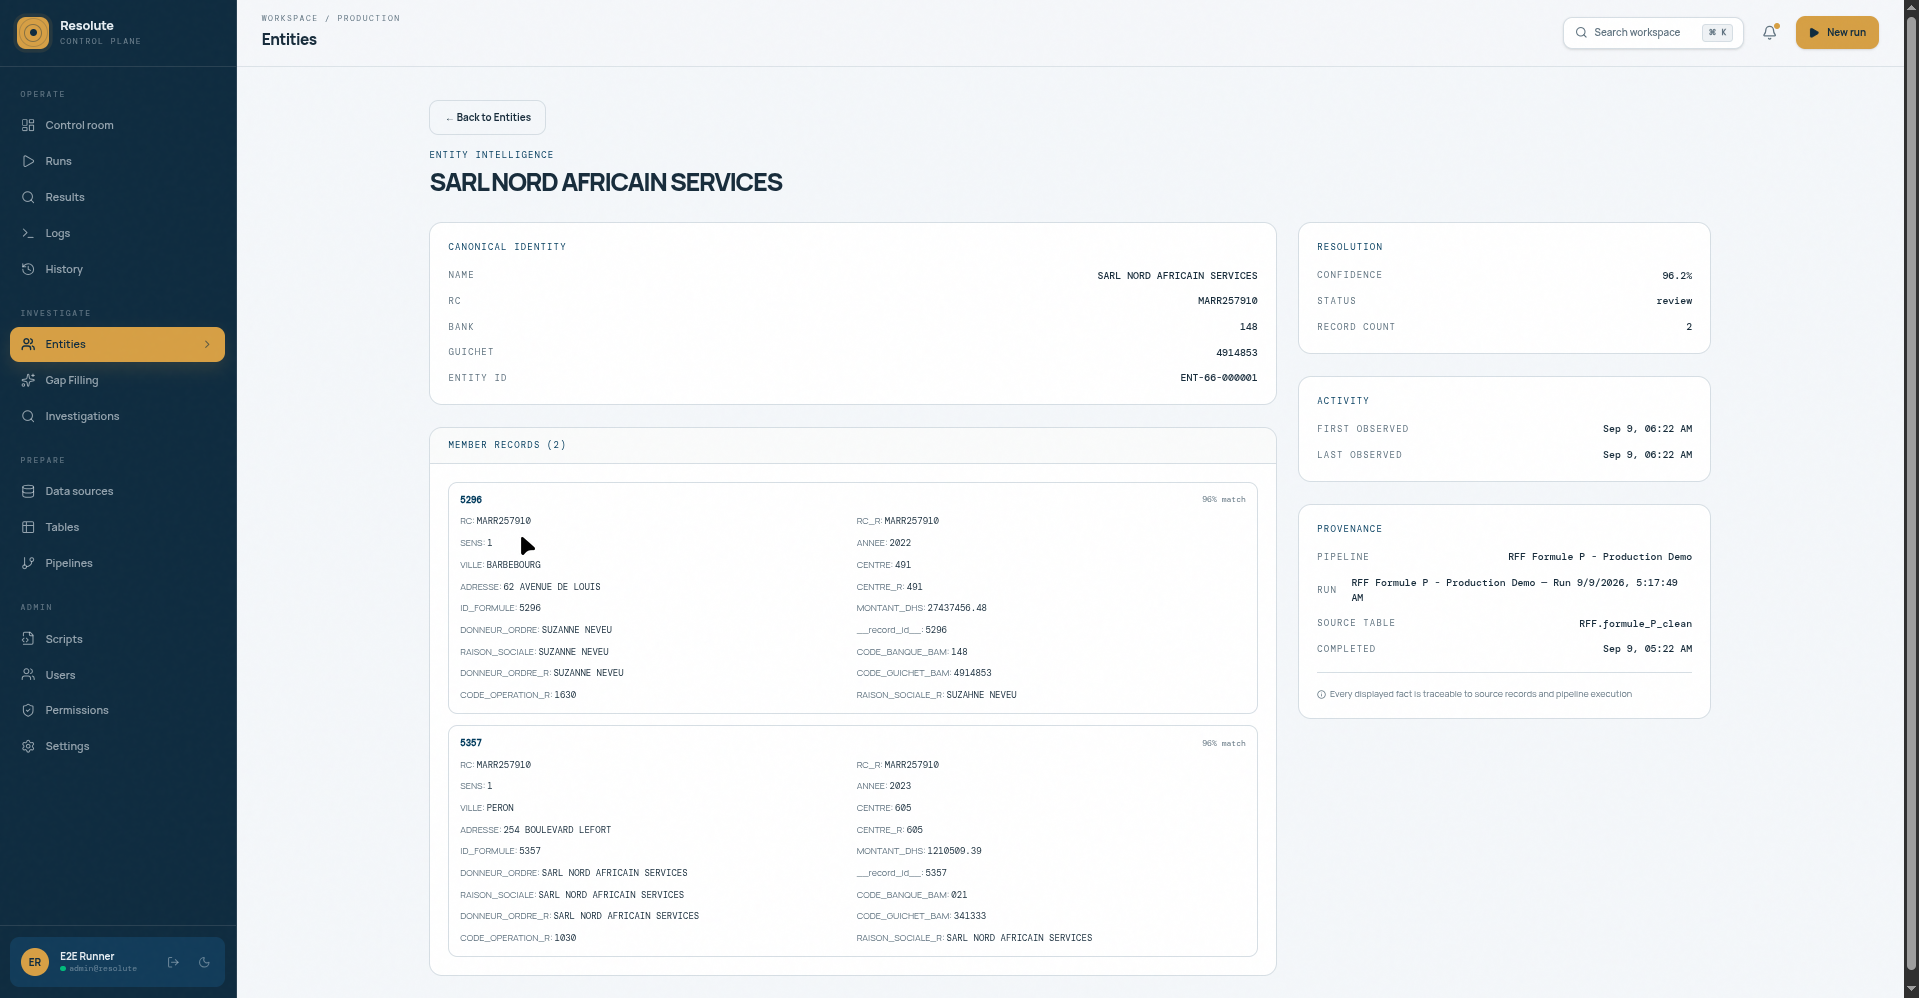
\includegraphics[width=0.9\textwidth]{images/screenshots/entity_details.png}
\caption{Fiche détaillée d'une entité : attributs canoniques et déclarations rattachées avec leurs champs.}
\label{fig:shot-entite}
\end{figure}

\subsection{Recherche intelligente d'opérateurs}

La barre de recherche constitue l'interface principale pour retrouver un opérateur. Elle accepte une requête unique en langage libre et détecte automatiquement le type de recherche : une requête purement numérique est interprétée comme un code de banque, une requête mixte comme un code de guichet, une requête au format du Registre de Commerce comme un identifiant, et toute autre requête comme un nom d'entreprise. La recherche combine l'indexation plein texte de la base avec des filtrages ciblés, en priorisant le nom canonique des entités puis les identifiants exacts. Un moteur de synonymes enrichit la requête avec les variantes connues, les résultats sont dédupliqués par entité, et le tri reflète la pertinence globale. Cette recherche permet ainsi de retrouver un opérateur même lorsque la requête ne reprend exactement aucune des formes stockées en base.

\section*{Conclusion}

Ce chapitre a présenté la transformation du pipeline en une plateforme opérationnelle : une architecture en couches séparées qui isole l'interface, la logique métier et le calcul ; un serveur d'API qui sécurise les accès et persiste l'état du système ; un worker qui exécute les traitements lourds avec un suivi temps réel ; et une interface qui rend l'ensemble accessible à des utilisateurs non informaticiens, de la configuration jusqu'à la recherche d'opérateurs. Le chapitre suivant évalue rigoureusement la qualité des résultats produits par cet ensemble.
